\section{Testing Reasoning in the Visual Domain}

% Slide 5: Testing Reasoning in the Visual Domain
\begin{frame}{CLEVR looked solved. It wasn't.}
  \begin{columns}
    \column{0.48\textwidth}
    \begin{itemize}
      \item Models reached 99%+ accuracy
      \item Visual question answering as a proxy for reasoning
      \item CLEVR reduced many trivial dataset biases
      \item CLEVR looked close to solved
      \item Question: did they really learn reasoning?
    \end{itemize}

    \column{0.52\textwidth}
    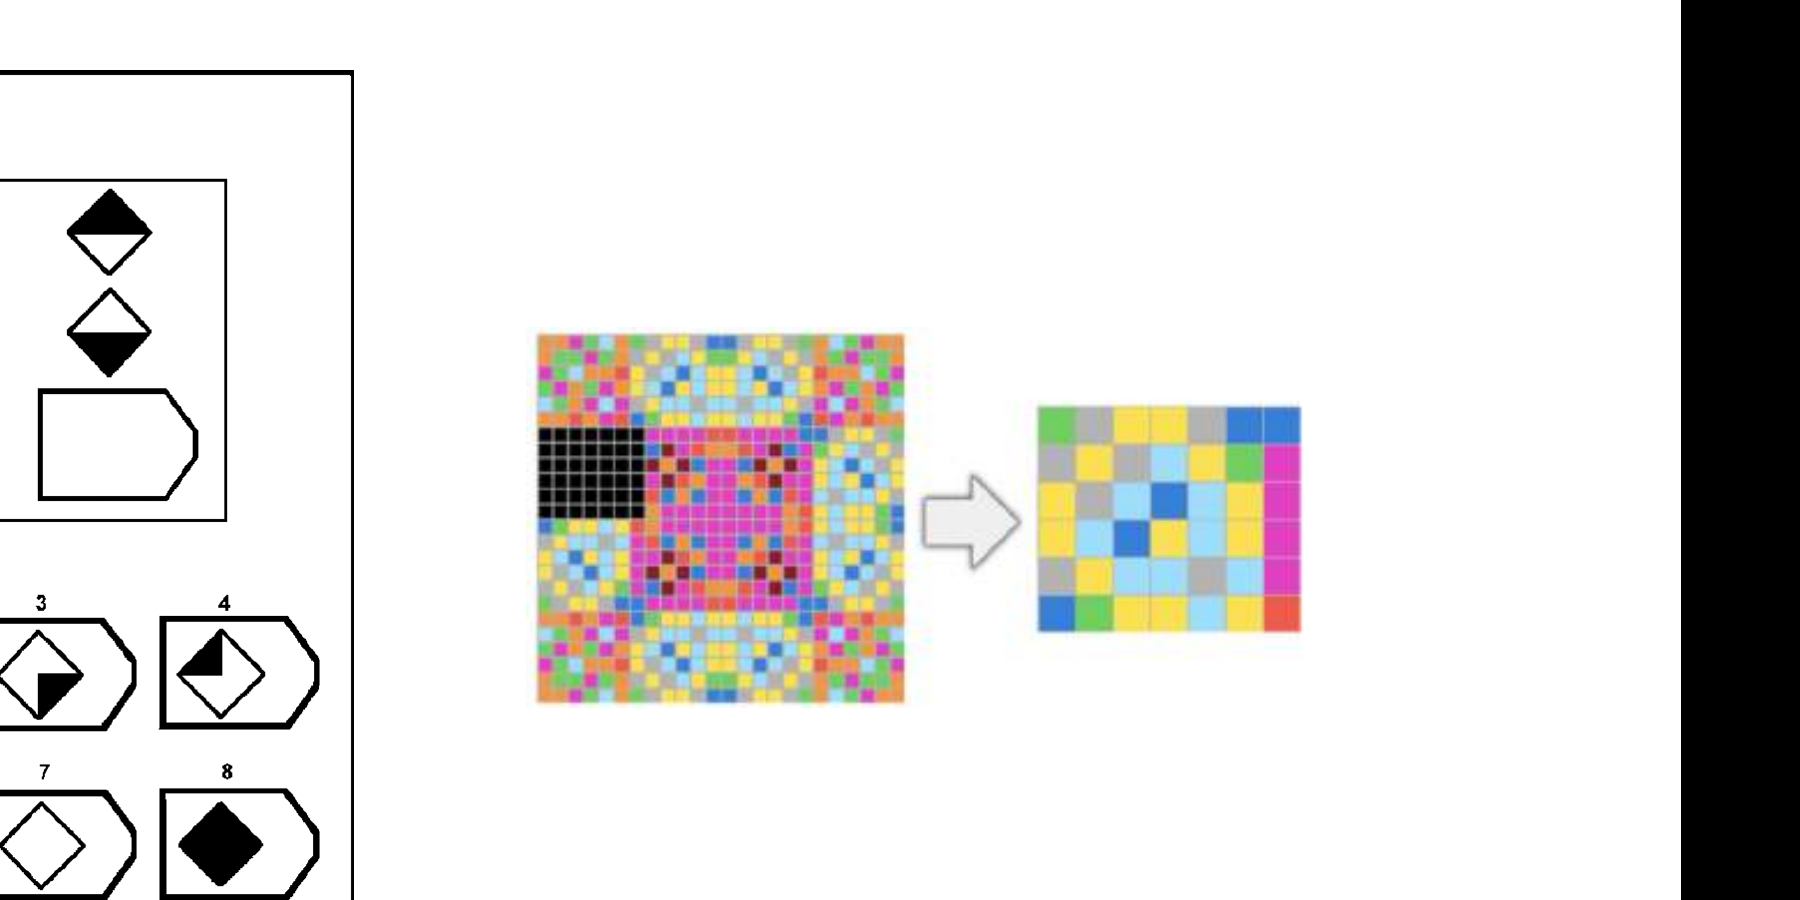
\includegraphics[width=\textwidth,height=0.6\textheight,keepaspectratio]{assets/clevr-scene-example}
    \vspace{-0.3em}
    {\tiny Source: CLEVR dataset (Johnson et al., CVPR 2017)}
  \end{columns}
  \note{I begin with vision because CLEVR was designed exactly for this kind of question. It is a controlled benchmark for compositional visual reasoning, and by the time of this work, several models looked close to solving it. So the natural next question was: are they actually reasoning, or are they still leaning on hidden shortcuts?}
\end{frame}

% Slide 6: A Two-Player Black-Box Test for VQA
\begin{frame}{A Two-Player Black-Box Test for VQA}
  \begin{itemize}
    \item Visual-QA Player answers the question
    \item Adversarial Player reconfigures the scene
    \item Enforcers keep the scene valid and answer-preserving
    \item If the answer changes, reasoning failed
  \end{itemize}
  \begin{center}
    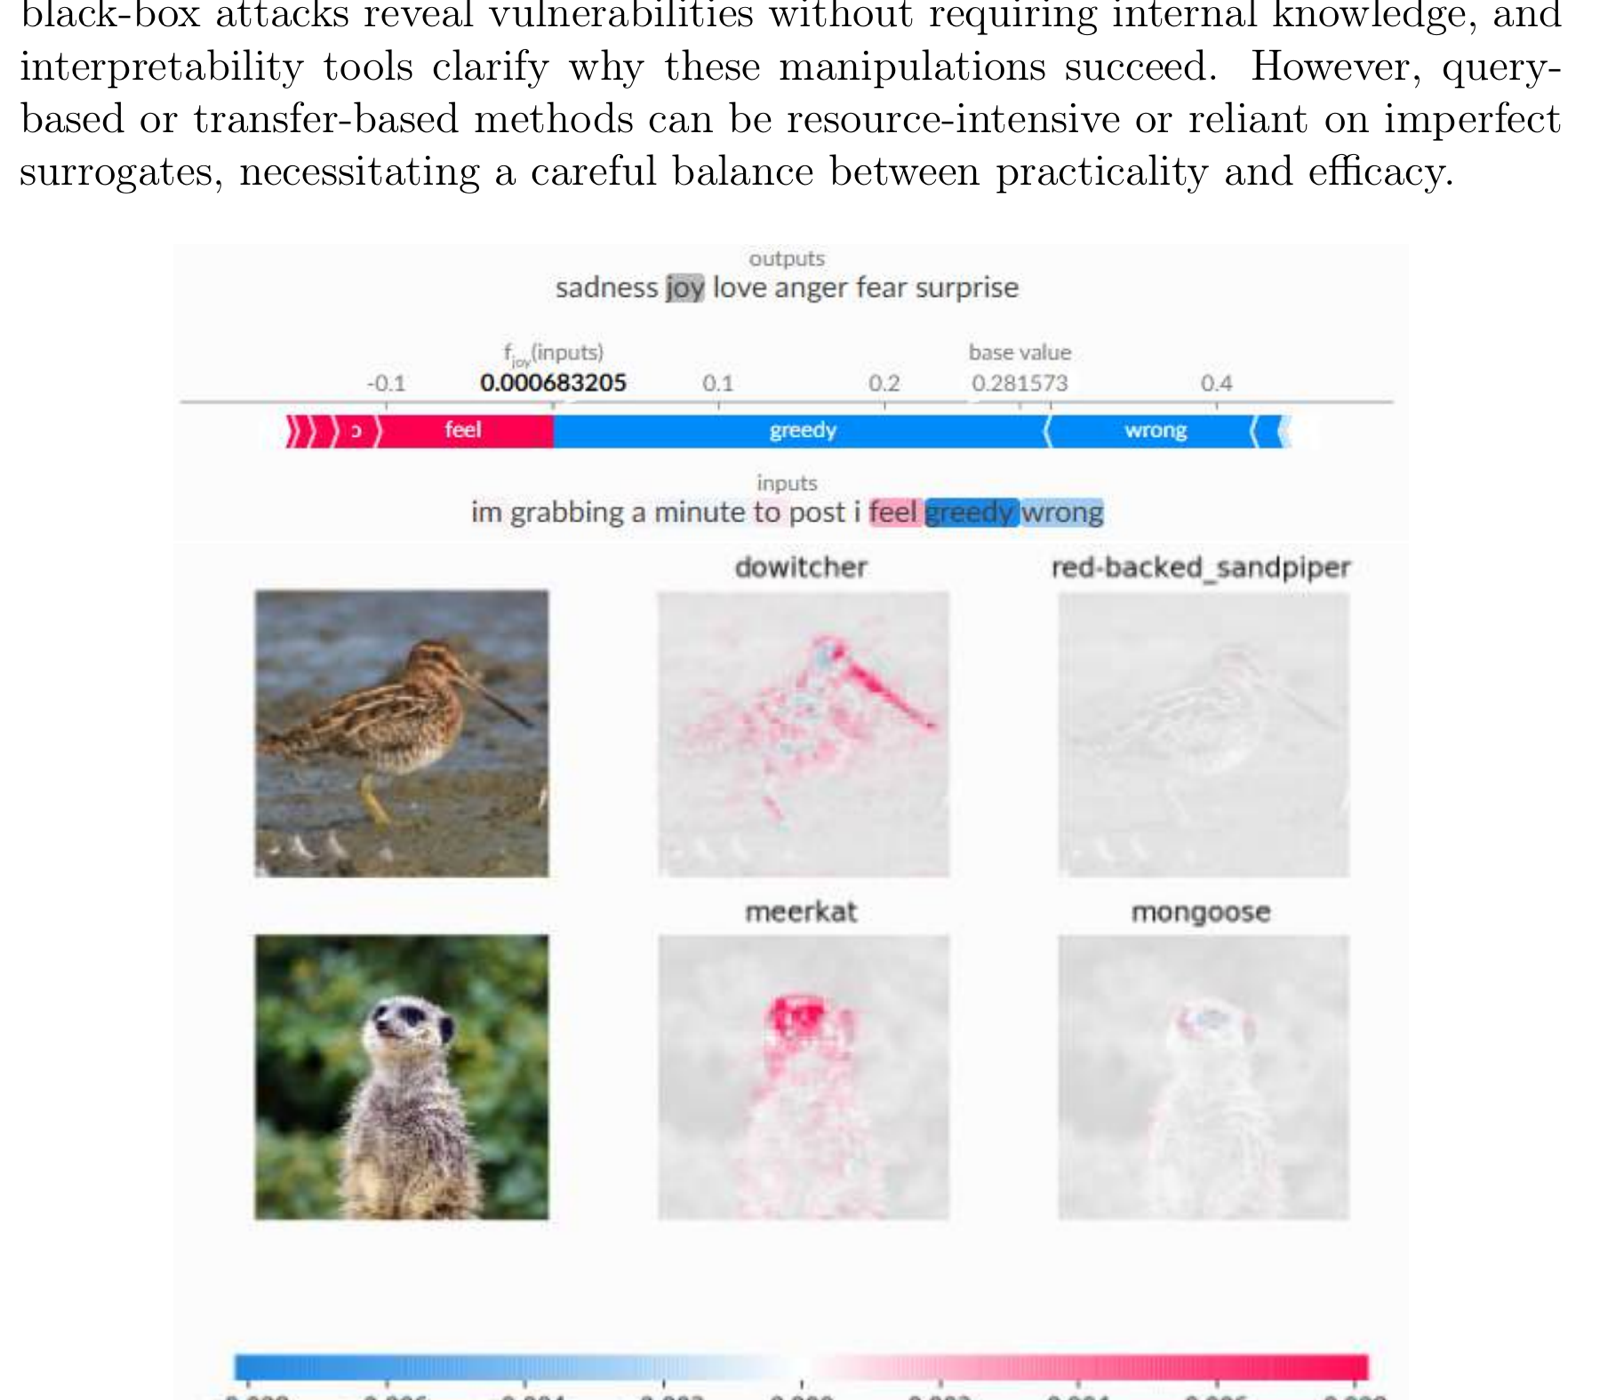
\includegraphics[width=0.8\textwidth,height=0.55\textheight,keepaspectratio]{assets/thesis-fig-2-1-two-player-game}
    \vspace{-0.3em}
    {\tiny Source: Thesis Fig. 2.1 / ICLR 2022 Fig. 1}
  \end{center}
  \note{The setup is a zero-sum game. One player is the model under test. The other is an adversarial scene manipulator. Crucially, the manipulator does not get gradients or model internals. It only changes the scene in ways that remain valid for the same question and answer. So this is not a pixel attack. It is a semantic black-box test of whether the model's reasoning is invariant under equivalent scene reconfigurations.}
\end{frame}

% Slide 7: Hero Slide — 99% accuracy. Still brittle.
\begin{frame}{99\% accuracy. Still brittle.}
  \begin{columns}[t]
    \column{0.23\textwidth}
    \begin{block}{FiLM}
      \centering
      \Large 96.2 \textrightarrow{} 48.0
      \normalsize
      \vspace{0.5em}

      (50\% drop)
    \end{block}

    \column{0.23\textwidth}
    \begin{block}{RN}
      \centering
      \Large 93.2 \textrightarrow{} 47.0
      \normalsize
      \vspace{0.5em}

      (50\% drop)
    \end{block}

    \column{0.23\textwidth}
    \begin{block}{TbD}
      \centering
      \Large 99.1 \textrightarrow{} 69.0
      \normalsize
      \vspace{0.5em}

      (30\% drop)
    \end{block}

    \column{0.23\textwidth}
    \begin{block}{MDetr}
      \centering
      \Large 99.7 \textrightarrow{} 60.0
      \normalsize
      \vspace{0.5em}

      (40\% drop)
    \end{block}
  \end{columns}

  \vspace{1em}
  \centering
  \textit{Near-perfect benchmark scores collapse under semantic perturbations}

  \note{These are state-of-the-art models that looked solved on CLEVR. FiLM drops from 96.2 to 48.0. RN from 93.2 to 47.0. Even MDetr at 99.7 drops to 60.0. Our black-box semantic manipulations reveal brittleness hidden by benchmark accuracy.}
\end{frame}

% Slide 8: Visual Chapter — Qualitative Failures
\begin{frame}{Small changes. Big failures.}
  \begin{itemize}
    \item Changes are small
    \item Changes are valid
    \item Humans usually see no reason the answer should change
    \item Yet the model flips its answer
  \end{itemize}
  \begin{center}
    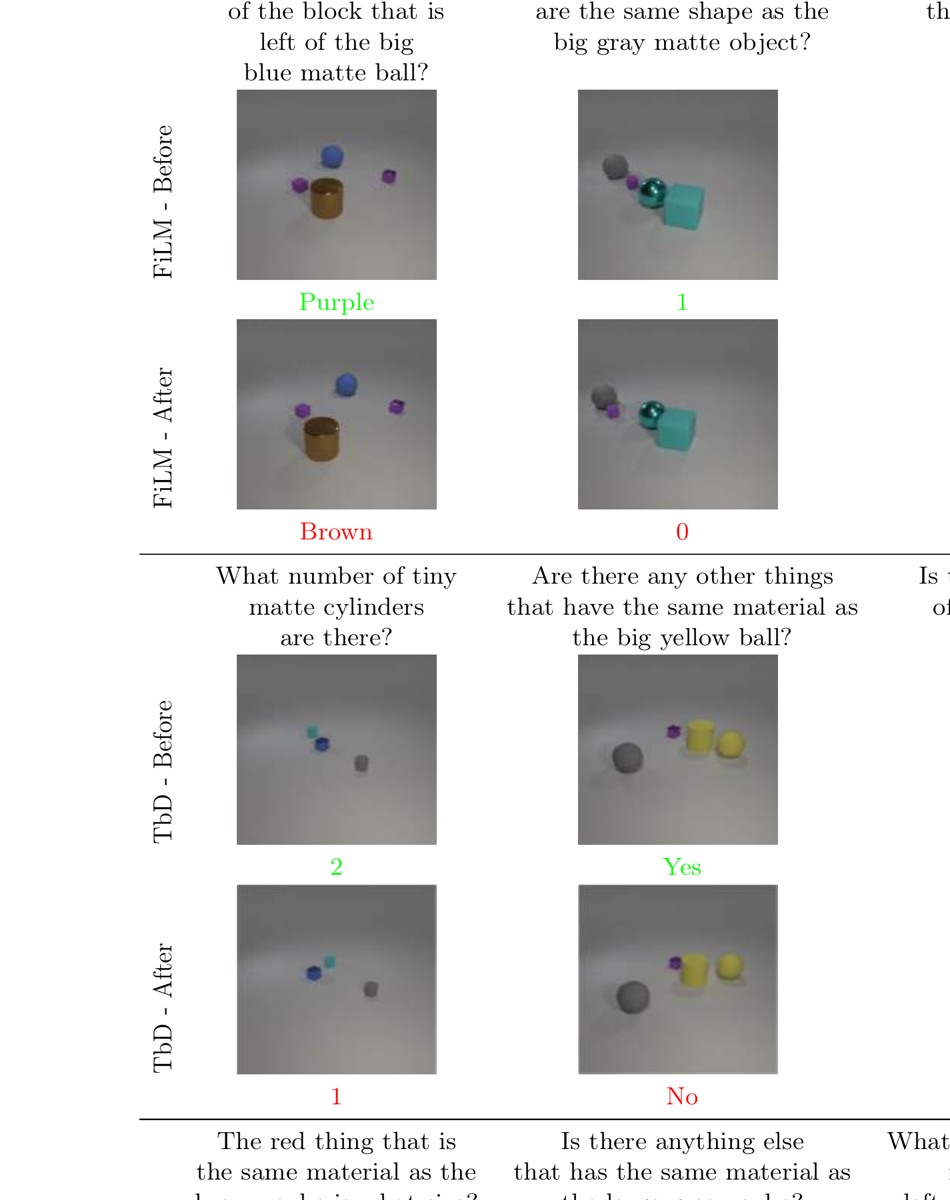
\includegraphics[width=0.85\textwidth,height=0.65\textheight,keepaspectratio]{assets/thesis-fig-2-2-visual-failures-tight}
    \vspace{-0.3em}
    {\tiny Source: Thesis Fig. 2.2 (tightly cropped for readability)}
  \end{center}
  \note{This is where the result becomes intuitive. The manipulations are not bizarre. They are small and semantically harmless. A human typically sees no reason the answer should change, but the model changes it anyway. In some cases, perception still looks fine, which suggests the failure is not only visual recognition. It is also a reasoning failure over the recognized content.}
\end{frame}

% Slide 9: What the Visual Chapter Proved
\begin{frame}{What the visual chapter proved}
  \begin{itemize}
    \item High accuracy $\neq$ robust reasoning
    \item Benchmark success hides brittleness
    \item Semantic stress-testing reveals real capabilities
  \end{itemize}
  \note{The visual chapter gave me the first thesis-level lesson: benchmark success is not proof of reasoning. It also showed that just adding more adversarially manipulated data is not a full solution. That led directly to the next question: if this pathology is real, does it also appear in language-based reasoning tasks like code generation?}
\end{frame}
